\documentclass[Main]{subfiles}

\begin{document}


\section{Designprocess}

\subsection{Fjernbetjening}

Projektet skulle indeholde en sender som kunne sende kommandoer til dronen.

\begin{figure}[H]
\centering
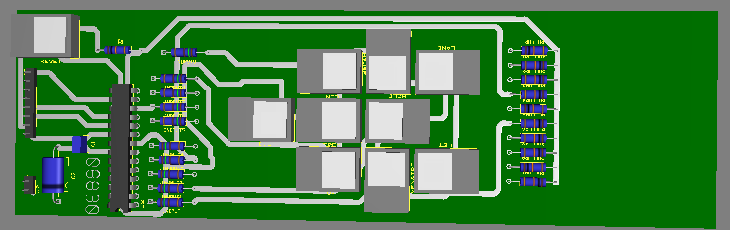
\includegraphics[width = 1 \textwidth]{3dUdenTal}
\caption{3D Figur af sender}
\label{Fig:3dUdenTal}
\end{figure}


Senderen som ses på figur \ref{Fig:3dUdenTal}, er bygget op i form som en fjernbetjening for, at det er muligt at betjene den med én hånd.
Fjernbetjeningen indeholder en µ-controller, radiosender og knapper.
Knapperne er her brugeren vælger et program/kommando der skal sendes til dronen. Når en knap bliver trykket ned, registrere µ-kontrolleren det. Denne genere så en frame med brugervalget. Denne frame bliver så sendt til radioen via SPI, hvorefter radioen får besked om at sende framen fra µ-kontrolleren.

\subsection{4+1 View}


\subsubsection*{Logic View}

Fjernbetjeningen udgør den største del af Use Casene beskrevet i kravspecifikationen\cite[s. 7 -- 11]{Kravspec}.

Et lille scenarie kunne optegnes og der kunne sættes nogle klasse navne på for, hvad der skulle være i de forskellige hardware-komponenter.

\begin{figure}[H]
\centering
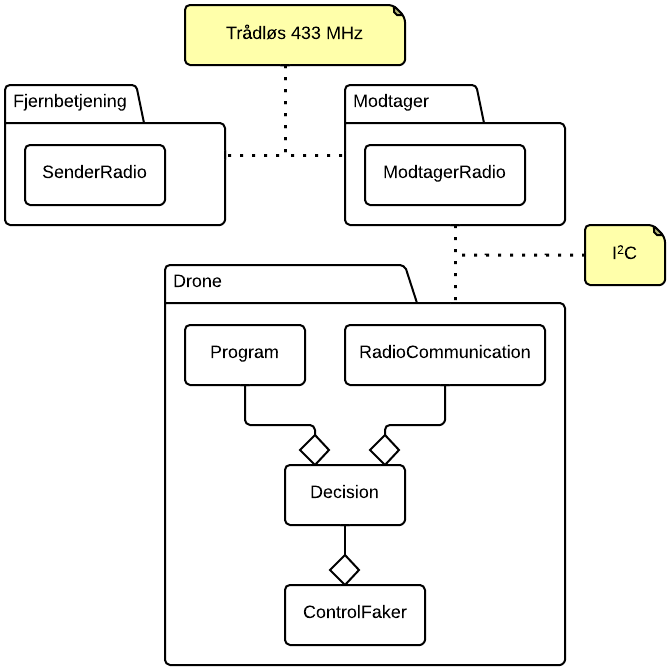
\includegraphics[width = 0.55 \textwidth]{Overview}
\caption{De første klasser}
\label{Fig:Overview}
\end{figure}


Ved at analysere diagrammet yderligere med flere Use Cases, blev der optegnet flere klasser og til sidst var der et klassediagram. 
Fra klasse diagrammet blev små sekvensdiagrammet herefter udtænkt, således forbindelsen fra fjernbetjeningen til dronen blev mere håndgribelig, vist på Figur \ref{Fig:sendProgram}.


\begin{figure}[H]
\centering
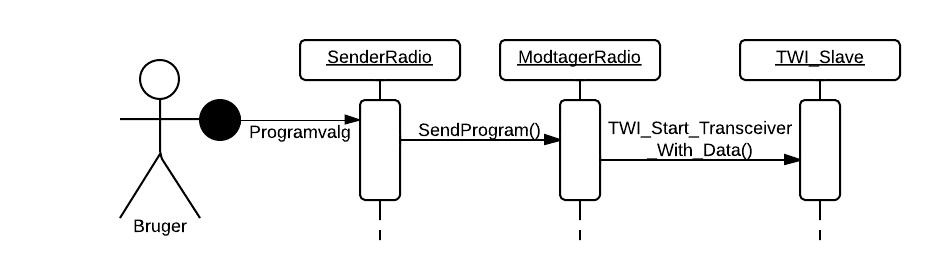
\includegraphics[width = 0.7 \textwidth]{SendProgram}
\caption{Sekvensdiagram fra fjernbetjening til drone.}
\label{Fig:sendProgram}
\end{figure}

\subsubsection*{Deployment View}

\begin{figure}[H]
\centering
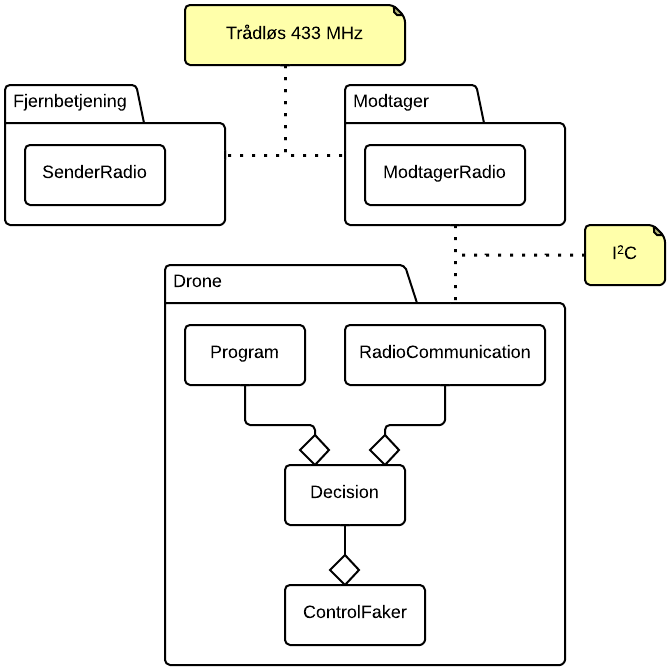
\includegraphics[width = 0.55 \textwidth]{Overview}
\caption{Intern kommunikation mellem enhederne.}
\label{Fig:Overview}
\end{figure}

Fjernbetjeningen sender en frame til dronen vha. det trådløse 433 MHz-signal, som opfanges af modtager-enheden.
Herefter bliver pakken lagt over i en output buffer til dronen som. Dronen kan så hente denne pakke når den har tid til det. Kommunikationen mellem dronen og modtagern er gennem \itoc protokollen.


\begin{figure}[H]
\centering
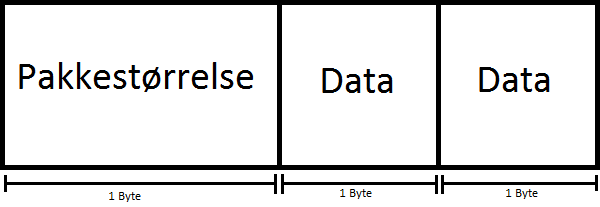
\includegraphics[width = 0.7 \textwidth]{PakkeUdenCrc}
\caption{Pakken fra fjernbetjæning til drone.}
\label{Fig:PakkeUdenCrc}
\end{figure}

Pakken der bliver sendt fra fjernbetjæningen over modtagern og til dronen ser ud som det ses på figur \ref{Fig:PakkeUdenCrc}.
Den første byte indeholder en indikation om det er et program der vælges.
Den anden byte er et nummer, som fortæller dronen hvad for et program der skal køres.






\subsubsection*{Process View}
Process view beskriver kommunikationen imellem de forskellige processer.

Dette projekt indeholder 3 processer, en på senderen, en på modtageren og en på dronen.

Processen på fjernbetjeningen snakker kun med radioen og det er normal SPI kommunikation. Der er ikke problemer med overskrivning af data der er ved at blive brugt af radioen.

Modtageren og dronen er to sideløbende processer der snakker sammen.
Modtageren modtager en frame fra senderen, som skal sendes over \itoc til dronen.

For at sikre at der ikke sker fejl, er der lagt en sikkerhed ind på modtageren. Modtageren og dronen deler 2 byte mellem sig.

Når modtageren har en ny pakke til dronen, tjekker den først om der er en \itoc transmission i gang. Hvis ikke bliver de nye data lagt over i output bufferen. Der bliver startet en svar funktion, så næste gang dronen spøger efter data kan den modtage de nyeste data.

\subsubsection*{Implementation View}
Koden til dronen, radiosenderen og radiomodtageren er skrevet i programmeringssproget C.

Der er tre projekter at arbejde videre på, beskrevet i næste afsnit.


\begin{itemize}
\item Sender
\item Modtager
\item Drone
\end{itemize}

Det er muligt at videreudvikle på projektet.
En udførlig guide til hvordan man kommer i gang med det, er at finde i  designdokumentet\cite[afs. 2.4]{Design}.















\end{document}
